% ============================================================
%  7.3. PREPARACIÓN DE LOS DATOS  -- parte del capítulo 7
%  ------------------------------------------------------------
%  Guía 2.7.3: (1) datos seleccionados y por qué, (2) limpieza,
%  faltantes y atípicos, (3) transformaciones y codificación,
%  (4) ingeniería y selección de características, (5) conjuntos
%  de entrenamiento y prueba. Justificar, no enumerar comandos.
%  Notebooks: 02_preprocesamiento.ipynb (limpieza, data/interim/)
%             03_feature_engineering.ipynb (variables, partición,
%             data/processed/tabla_modelado.parquet)
% ============================================================
\section{Preparación de los datos}
\label{sec:preparacion-datos}

La preparación convierte las fuentes crudas en el conjunto de datos H3 sobre el que se modela.
Aplica, en el orden fijado por la sección~\ref{sec:hallazgos-decisiones}, los criterios que
el análisis exploratorio solo había medido. Se ejecuta en dos notebooks:
\begin{itemize}
  \item \var{02_preprocesamiento} limpia las consultas y construye el conjunto de datos H3 por zona, que
        guarda en \var{data/interim/}.
  \item \var{03_feature_engineering} añade las variables, declara cuáles serán predictores y
        reserva el conjunto de prueba. Su resultado es
        \var{data/processed/tabla_modelado.parquet}, con 1.628 filas y 18 columnas.
\end{itemize}
Todos los umbrales viven en un único archivo de configuración (\var{config.py}), de modo
que ninguna cifra se escribe a mano dentro de los notebooks.

\subsection{Selección de los datos}
\label{sec:seleccion-datos}

Se seleccionan tres conjuntos, cada uno por una razón distinta.

\textbf{Consultas.} Se conservan todas las consultas válidas del período completo, sin
muestreo. El problema se formula sobre el total acumulado por zona
(capítulo~\ref{cap:problema}), y descartar semanas o usuarios reduciría la información de
las zonas con poca actividad, que son precisamente las de interés.

\textbf{Zonas.} El conjunto de datos H3 se construye como la unión de dos conjuntos: las celdas
de Kontur cuyo centroide cae dentro del área de estudio (1.577) y las celdas donde se
originó al menos una consulta válida. Esta unión es deliberada. Si solo se tomaran las
zonas con consultas, desaparecerían las 611 zonas pobladas sin ninguna consulta, que son
el tipo de zona que el proyecto debe poder señalar. Si solo se tomaran las celdas de
Kontur, se perderían 51 zonas con consultas situadas en el borde del área. El resultado
son 1.628 zonas: 1.017 con consultas y 611 pobladas sin consultas
(figura~\ref{fig:consultas-por-zona}).

\begin{figure}[H]
  \centering
  \caption{Consultas por zona y zonas pobladas sin consultas}
  \label{fig:consultas-por-zona}
  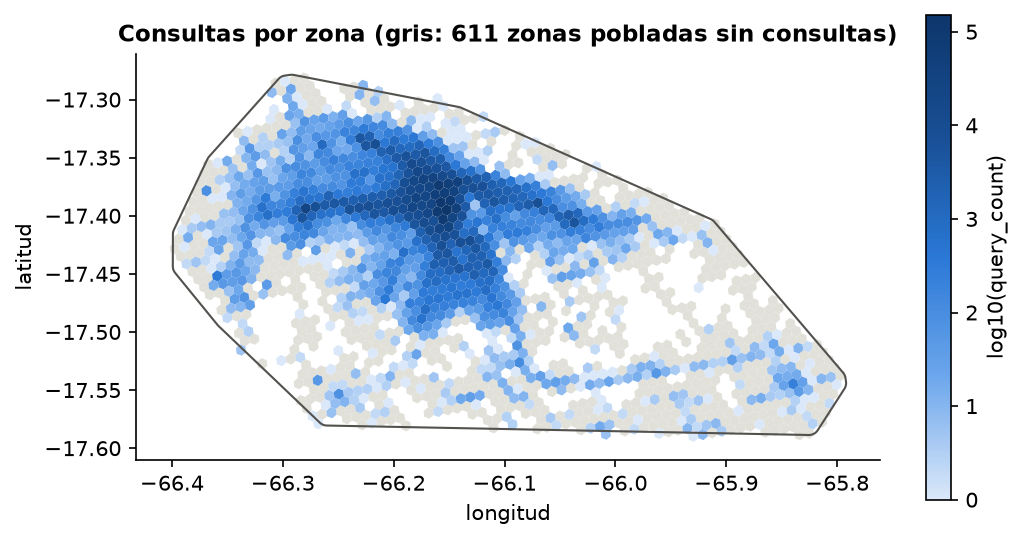
\includegraphics[width=0.85\textwidth]{imagenes/07_desarrollo/7_3_preparacion/consultas_por_zona.png}
  \fuente{Elaboración propia, a partir de \var{02_preprocesamiento} (sección 8). Escala de
  color: $\log_{10}$ del conteo; gris: zonas pobladas sin consultas.}
\end{figure}

Las zonas sin consultas no se distribuyen al azar: se concentran en la periferia del
valle y en el sur del área, lejos del núcleo donde el color es más intenso. Si se
eliminaran, la tabla describiría solo el territorio donde la aplicación ya se usa.

\textbf{Zonas del modelo.} De las 1.628 zonas, entran al modelo las que tienen al menos
10 habitantes, que son 1.381. La tabla~\ref{tab:zonas-modelo} muestra qué se excluye. El
motivo es técnico: el modelo estima una tasa por habitante, y con muy pocos habitantes esa
tasa se vuelve inestable (una sola consulta en una zona de 2 habitantes equivale a 500 por
cada 1.000). Las zonas sin población no pueden entrar, porque la exposición sería cero. La
exclusión apenas afecta al volumen: se pierden 242 consultas, y el modelo conserva
1.924.336 de las 1.924.578 consultas válidas (el 99,99~\%).

\begin{table}[H]
  \centering
  \caption{Zonas del área de estudio según su población}
  \label{tab:zonas-modelo}
  \interlineadoSimple
  \small
  \begin{tabular}{@{}lrr@{}}
    \toprule
    \textbf{Grupo} & \textbf{Zonas} & \textbf{Consultas} \\
    \midrule
    Sin población en Kontur (\var{population} $= 0$) & 43 & 102 \\
    Entre 1 y 9 habitantes & 204 & 140 \\
    \textbf{Al menos 10 habitantes (zonas del modelo)} & \textbf{1.381} & \textbf{1.924.336} \\
    \midrule
    Total & 1.628 & 1.924.578 \\
    \bottomrule
  \end{tabular}
  \fuente{Elaboración propia, a partir de
  \var{resultados/03_feature_engineering/zonas_por_grupo.csv}.}
\end{table}

La población total de las 1.628 zonas es de 1.226.308 habitantes, algo más que los
1.223.871 de las celdas de Kontur situadas dentro del área
(sección~\ref{sec:area-estudio}). La diferencia, de 2.437 habitantes, proviene de las
zonas de borde incorporadas por tener consultas: su centroide queda fuera del contorno,
pero Kontur les asigna población.

\subsection{Limpieza, datos faltantes y valores atípicos}
\label{sec:limpieza}

\textbf{Consolidación.} Los 85 archivos, que cubren 84 semanas con datos (una semana viene
partida en dos archivos; sección~\ref{sec:cobertura-temporal}), se leen con detección automática de codificación:
se intenta UTF-8 y, si falla, Latin-1. Así se leen correctamente los seis archivos del
lote 2024 y los nombres con tildes (por ejemplo, ``Santivañez''). Las columnas
equivalentes de ambos esquemas se unifican, y a cada fila se le añade su linaje. Las
consultas se ordenan de forma estable (archivo, marca de tiempo, usuario y coordenadas),
para que cualquier ejecución produzca exactamente el mismo resultado.

\textbf{Filtros.} Se aplican seis filtros en un orden fijo, que va de lo inequívoco a lo
que depende de decisiones. La tabla~\ref{tab:flujo-filtros} y la
figura~\ref{fig:flujo-limpieza} muestran cuántas consultas elimina cada paso.

\begin{table}[H]
  \centering
  \caption{Flujo de limpieza de las consultas}
  \label{tab:flujo-filtros}
  \interlineadoSimple
  \small
  \begin{tabularx}{\textwidth}{@{}clrrY@{}}
    \toprule
    \textbf{Paso} & \textbf{Regla} & \textbf{Eliminadas} & \textbf{Quedan} & \textbf{Justificación} \\
    \midrule
    0 & Consultas crudas & --- & 1.927.675 & --- \\
    1 & Origen en (0,0) & 3 & 1.927.672 & Coordenadas no localizables \\
    2 & Origen fuera de Bolivia & 9 & 1.927.663 & Coordenadas imposibles para el servicio \\
    3 & Copia de duplicado exacto & 60 & 1.927.603 & Se conserva la primera aparición \\
    4 & Origen fuera del área & 2.509 & 1.925.094 & Área fijada en la sección~\ref{sec:area-estudio} \\
    5 & Distancia $>$ 50~km & 283 & 1.924.811 & Fuera de la escala urbana (sección~\ref{sec:atipicos}) \\
    6 & Usuario anómalo & 233 & 1.924.578 & Al menos 2 de 6 señales (sección~\ref{sec:atipicos}) \\
    \bottomrule
  \end{tabularx}
  \fuente{Elaboración propia, a partir de
  \var{resultados/02_preprocesamiento/flujo_limpieza.csv}. Se conserva el 99,84~\% de las
  consultas.}
\end{table}

\begin{figure}[H]
  \centering
  \caption{Consultas eliminadas en cada paso de la limpieza}
  \label{fig:flujo-limpieza}
  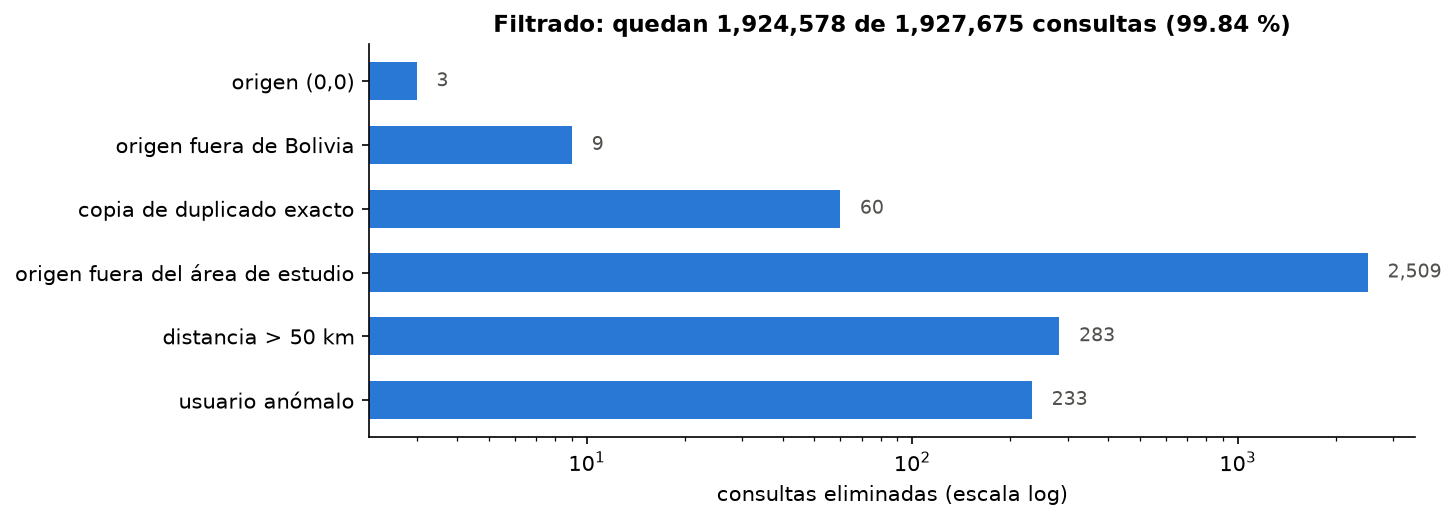
\includegraphics[width=0.9\textwidth]{imagenes/07_desarrollo/7_3_preparacion/flujo_limpieza.png}
  \fuente{Elaboración propia, a partir de \var{02_preprocesamiento} (sección 5). Eje
  horizontal en escala logarítmica.}
\end{figure}

El orden importa por dos motivos. Primero, los filtros geográficos inequívocos (pasos 1 y
2) van antes que la detección de duplicados, para que las coordenadas imposibles no
cuenten como consultas válidas. Segundo, el área de estudio (paso 4) se delimitó con los
orígenes de usuarios no anómalos y \emph{sin} aplicar el umbral de distancia, de modo que
los dos criterios no se contaminan entre sí. La mayor exclusión, la de consultas fuera del
área, representa apenas el 0,13~\% del total. En conjunto, la limpieza no altera la
estructura de los datos: corrige errores puntuales. Las cifras coinciden exactamente con
las que midió el análisis exploratorio, porque ambos notebooks usan las mismas funciones.

\textbf{Datos faltantes.} La limpieza no imputa ningún valor, por tres razones:
\begin{itemize}
  \item Las columnas que usa el proyecto no tienen nulos
        (sección~\ref{sec:datos-faltantes-eda}).
  \item Las 611 zonas pobladas sin consultas reciben un conteo de 0, que es su valor
        observado. No se trata como faltante.
  \item Las 43 zonas con consultas pero sin registro en Kontur reciben población 0. Es una
        ausencia estructural de la fuente, no un dato que deba estimarse; esas zonas quedan
        fuera del modelo por el umbral de población.
\end{itemize}
Las siete semanas sin datos tampoco se rellenan. Se registran para calcular las semanas
realmente observadas (sección~\ref{sec:transformaciones}).

\textbf{Valores atípicos.} Solo se eliminan los atípicos que representan errores o un uso
no humano: la distancia de más de 50~km y los usuarios anómalos. Los valores extremos
legítimos se conservan. Por ejemplo, la zona con más consultas acumula 152.494, frente a
una mediana de 6. Esas zonas son reales, están en el centro de la ciudad y forman parte
del fenómeno. Su efecto se controla con métricas y modelos propios de datos de conteo, no
eliminándolas.

\subsection{Transformaciones y codificación de variables}
\label{sec:transformaciones}

Las transformaciones convierten consultas individuales en un conjunto de datos H3 por zona y dejan cada
variable en la escala que requieren los modelos. La tabla~\ref{tab:transformaciones} las
resume con su justificación.

\begin{table}[H]
  \centering
  \caption{Transformaciones y codificación aplicadas}
  \label{tab:transformaciones}
  \interlineadoSimple
  \small
  \begin{tabularx}{\textwidth}{@{}L{0.26\textwidth}L{0.34\textwidth}Y@{}}
    \toprule
    \textbf{Transformación} & \textbf{Qué hace} & \textbf{Por qué} \\
    \midrule
    Asignación de zona & Convierte las coordenadas de origen en su celda H3 de resolución~8 (\var{h3_origin}) & Unidad de análisis común con Kontur, sin reproyección (sección~\ref{subsec:h3}) \\
    Agregación & Cuenta las consultas por zona de origen (\var{query_count}) & La variable objetivo es el total del período \\
    Bloque espacial & Asigna a cada zona su celda madre H3 de resolución~6 (\var{block_id}), de unos 36~km\textsuperscript{2} & Unidad de validación y de reserva de prueba \\
    Semanas equivalentes observadas & $W_{obs} = \text{días con datos} / 7 = 568/7 = 81{,}143$ & Expresar lo esperado por semana sin contar el hueco \\
    Exposición & $\log(\text{population})$ como \emph{offset} (coeficiente fijo igual a 1) & Modelar la tasa por habitante (sección~\ref{subsec:glm-poisson}) \\
    Escala de población & $\log(1 + x)$ en \var{pop_ring1} dentro de los modelos & Reduce la asimetría; no depende de los datos, así que no filtra información \\
    Municipio & Municipio más frecuente entre los orígenes de la zona; sin consultas, el de las zonas vecinas etiquetadas más cercanas & Estrato de la línea base B1 \\
    Anillo de distancia & Cuatro anillos (A1 a A4) según los cuartiles de la distancia media de cada bloque a la Plaza & Estrato de la línea base B2 y del sorteo de prueba \\
    \bottomrule
  \end{tabularx}
  \fuente{Elaboración propia, a partir de \var{src/features.py}, \var{src/modelos.py},
  \var{src/limpieza.py} y \var{resultados/02_preprocesamiento/metricas.json}.}
\end{table}

\textbf{Semanas equivalentes observadas ($W_{obs}$).} Hubo datos 538 días antes del hueco
y 30 después, 568 días en total, que equivalen a 81,143 semanas. Todos los modelos estiman
el total del período. Para comunicar el resultado a la organización en una unidad
intuitiva (consultas por semana), ese total se divide por $W_{obs}$ y no por las 91
semanas calendario. Dividir por 91 subestimaría el ritmo semanal, porque contaría semanas
en las que no se registró nada.

\textbf{Codificación de las variables categóricas.} El municipio y el anillo no se
convierten en variables indicadoras (\emph{one-hot}), porque ningún modelo los usa como
predictores. Sirven para definir los estratos de dos líneas base, que calculan una tasa
separada por grupo.

La etiqueta de municipio proviene del campo \var{origin_municipio} de las exportaciones de
Trufi Association, no de límites oficiales, y queda asignada a 14 municipios
(tabla~\ref{tab:municipios}). El municipio figura como ``Cochabamba'' en los datos, pero
corresponde a Cercado. Para comprobar si esa etiqueta es coherente dentro de cada zona, se
verificó su pureza. El 99,38~\% de las consultas comparte la etiqueta modal de su zona. Solo
el 5,02~\% de las zonas con consultas es de municipio \emph{mixto}, es decir, tiene menos
del 90~\% de sus consultas con la etiqueta modal. El único caso llamativo, Arani (50~\%),
corresponde a una zona con apenas dos consultas.

Esta decisión es aceptable para el propósito del proyecto porque el municipio se usa
únicamente como estrato en la línea base B1, que no fue la técnica seleccionada; ningún
modelo que participa en la selección final lo usa como predictor. Los resultados se
guardan en \var{resultados/03_feature_engineering/resumen_municipio.csv} y en
\var{metricas.json} (\var{pct_consultas_municipio_modal},
\var{pct_zonas_municipio_mixto}).

\begin{table}[H]
  \centering
  \caption{Zonas del modelo por municipio asignado y pureza de la etiqueta}
  \label{tab:municipios}
  \interlineadoSimple
  \small
  \begin{tabular}{@{}lrrrrr@{}}
    \toprule
    \textbf{Municipio} & \textbf{Zonas} & \textbf{Consultas} & \textbf{Población} & \textbf{\celda{\% consultas con\\etiqueta modal}} & \textbf{\celda{Zonas\\mixtas}} \\
    \midrule
    Cochabamba (Cercado) & 318 & 1.662.310 & 622.120 & 99,69 & 13 \\
    Sacaba & 259 & 90.113 & 180.427 & 99,99 & 1 \\
    Quillacollo & 137 & 65.275 & 146.291 & 97,71 & 12 \\
    Colcapirhua & 35 & 53.209 & 47.652 & 97,17 & 5 \\
    Tiquipaya & 47 & 46.785 & 60.991 & 92,27 & 7 \\
    Vinto & 89 & 3.403 & 56.167 & 95,53 & 4 \\
    Sipe Sipe & 92 & 1.357 & 35.950 & 99,78 & 2 \\
    Arbieto & 86 & 546 & 17.368 & 97,99 & 1 \\
    Villa Punata & 74 & 488 & 23.430 & 100,00 & 0 \\
    Tolata & 37 & 302 & 5.115 & 100,00 & 0 \\
    Villa Santivañez & 79 & 300 & 4.163 & 100,00 & 0 \\
    Villa José Quintín Mendoza & 76 & 170 & 13.386 & 99,41 & 1 \\
    Cliza & 47 & 76 & 11.604 & 100,00 & 0 \\
    Arani & 5 & 2 & 1.015 & 50,00 & 1 \\
    \midrule
    Total & 1.381 & 1.924.336 & 1.225.679 & 99,38 & 47 \\
    \bottomrule
  \end{tabular}
  \fuente{Elaboración propia, a partir de
  \var{resultados/03_feature_engineering/resumen_municipio.csv} y \var{metricas.json}. Zona
  mixta: menos del 90~\% de sus consultas con la etiqueta modal.}
\end{table}

La tabla muestra por qué el área de estudio excede los siete municipios del eje
metropolitano mencionados en el alcance. La componente contigua de orígenes se extiende
hacia el valle alto y el sur (Arbieto, Santivañez, Punata, Cliza, Tolata). Esos
municipios aportan muchas zonas pobladas, pero casi ninguna consulta. Cercado concentra el
86~\% de las consultas con el 51~\% de la población.

\subsection{Ingeniería y selección de características}
\label{sec:ingenieria-caracteristicas}

Cada columna del conjunto de datos H3 tiene un papel declarado antes de modelar. La
tabla~\ref{tab:grupos-variables} organiza las variables por su uso. Distinguir estos
papeles es la principal salvaguarda contra la fuga de información
(sección~\ref{subsec:fuga-datos}).

\begin{table}[H]
  \centering
  \caption{Variables del conjunto de datos H3 según su papel}
  \label{tab:grupos-variables}
  \interlineadoSimple
  \small
  \begin{tabularx}{\textwidth}{@{}L{0.18\textwidth}L{0.28\textwidth}Y@{}}
    \toprule
    \textbf{Papel} & \textbf{Variables} & \textbf{Uso} \\
    \midrule
    Objetivo & \var{query_count} & Lo que se estima: total de consultas de la zona en el período \\
    Exposición & \var{population} & Entra como \emph{offset} $\log(\text{population})$: convierte el conteo en una tasa por habitante \\
    Predictores & \var{dist_centro_km}, \var{pop_ring1} & Únicas variables explicativas de los modelos M1 a M3 \\
    Contraste & \var{dist_trazado_m}, \var{gtfs_covered} & Solo para interpretar la brecha; nunca entran a un modelo \\
    Grupos y validación & \var{municipality}, \var{distance_ring}, \var{block_id}, \var{in_test} & Estratos de las líneas base, pliegues de validación y marca de prueba \\
    Apoyo & \var{h3_cell}, \var{lat}, \var{lon}, \var{in_model}, \var{user_count}, conteos antes y después del hueco & Identificación, mapas, universo del modelo y análisis de sensibilidad \\
    \bottomrule
  \end{tabularx}
  \fuente{Elaboración propia, a partir de \var{config.py} (\var{PREDICTORES},
  \var{CONTRASTE}) y \var{03_feature_engineering} (secciones 3 a 7).}
\end{table}

La construcción de las variables sigue cuatro decisiones:

\textbf{Centro de referencia exógeno.} La distancia al centro (\var{dist_centro_km}) se
mide como distancia geodésica desde el centroide de cada zona hasta la Plaza 14 de
Septiembre, un punto fijado desde fuera de los datos. Como se vio en la
sección~\ref{sec:relaciones-variables}, este centro se asocia con las consultas mucho más
que el centroide del área. Tiene además una ventaja metodológica: al no calcularse con los
datos, no cambia entre pliegues de validación ni puede filtrar información de las zonas de
prueba.

\textbf{Población del entorno.} \var{pop_ring1} suma la población de las seis zonas del
primer anillo H3 alrededor de cada zona, sin incluirla a ella. \var{pop_ring2} hace lo
mismo con el segundo anillo. Ambas se calculan con la cobertura completa de Kontur para
Bolivia, y no solo con el área de estudio. Así, las zonas de borde no ven su entorno
artificialmente vacío. Estas variables capturan la densidad del vecindario, un indicador
indirecto de la concentración de actividades.

\textbf{Selección por colinealidad.} La figura~\ref{fig:correlacion-predictores} muestra
la correlación de Spearman entre los predictores candidatos. \var{pop_ring1} y
\var{pop_ring2} tienen una correlación de 0,954: aportan prácticamente la misma
información, e incluir ambas inflaría la varianza de los coeficientes sin mejorar la
estimación. Se conserva \var{pop_ring1}, que describe el entorno más inmediato y se asocia
un poco más con el conteo (0,836 frente a 0,804). La población de la propia zona no
aparece como predictor porque ya entra como exposición.

\begin{figure}[H]
  \centering
  \caption{Correlación de Spearman entre los predictores candidatos}
  \label{fig:correlacion-predictores}
  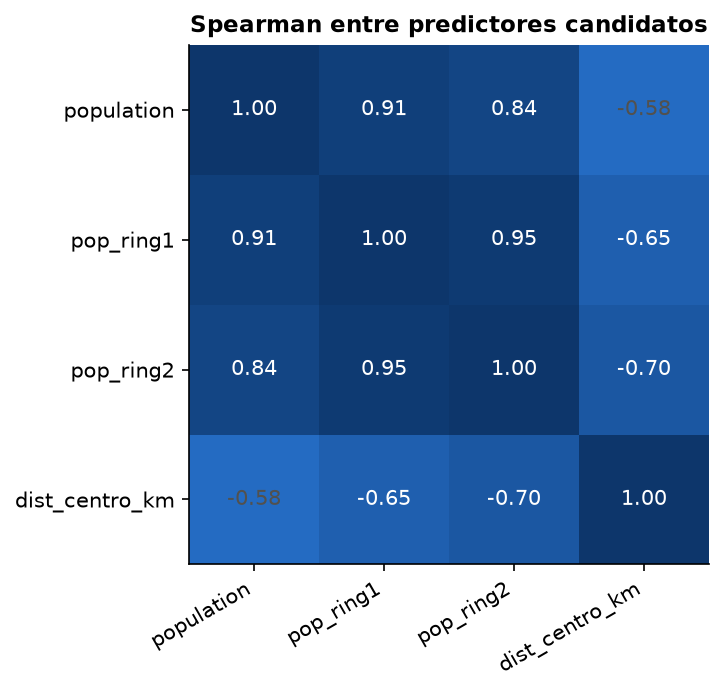
\includegraphics[width=0.5\textwidth]{imagenes/07_desarrollo/7_3_preparacion/correlacion_predictores.png}
  \fuente{Elaboración propia, a partir de
  \var{resultados/03_feature_engineering/correlacion_predictores.csv}.}
\end{figure}

\textbf{Exclusión de la cobertura.} \var{dist_trazado_m} es la distancia del centroide de
la zona al trazado GTFS más cercano, calculada en proyección métrica UTM 19S.
\var{gtfs_covered} vale 1 si esa distancia es de 500~m o menos. Con ese criterio, 634 de
las 1.628 zonas están cubiertas (626 de las 1.381 zonas del modelo). Ambas variables se
excluyen expresamente de los predictores
(secciones~\ref{sec:traduccion-necesidad} y~\ref{sec:area-estudio}), y el notebook de
modelado verifica que ninguna técnica las use. La cobertura se mide contra el trazado y no
contra las paradas, por la naturaleza del paratránsito (sección~\ref{subsec:gtfs}).

Con estas decisiones, el conjunto de predictores queda reducido a dos variables:
\var{dist_centro_km}, que resume la localización, y \var{pop_ring1}, que resume el
entorno. Es un conjunto deliberadamente pequeño. Con 1.381 zonas y una autocorrelación
fuerte, el número efectivo de observaciones independientes es mucho menor que el nominal,
y cada predictor adicional aumenta el riesgo de sobreajuste. Además, ambas variables son
exógenas: ninguna se calcula a partir de las consultas.

\subsection{Conjuntos de entrenamiento y prueba}
\label{sec:conjuntos-entrenamiento-prueba}

El conjunto de prueba se reserva en esta fase, antes de ajustar cualquier modelo, y se usa
una sola vez en la evaluación. La reserva no se hace por zonas individuales sino por
\emph{bloques} H3 de resolución~6: por la autocorrelación documentada en la
sección~\ref{sec:relaciones-variables}, una zona de prueba rodeada de vecinas de
entrenamiento sería casi una copia de ellas, y el error medido resultaría optimista
(sección~\ref{subsec:validacion-espacial}).

Las 1.381 zonas del modelo se reparten en 53 bloques. Para que la prueba represente todo el
gradiente centro-periferia, el sorteo se estratifica por anillo de distancia: en cada
anillo se reserva el 20~\% de sus bloques, con la semilla fija 42. Los cortes entre anillos
(12,52, 18,65 y 22,92~km de la Plaza) son los cuartiles de la distancia media de los
bloques, de modo que cada anillo tiene un número parecido de bloques. El sorteo solo usa la
geometría de los bloques y su anillo: ninguna consulta interviene en la selección.

\begin{table}[H]
  \centering
  \caption{Zonas del modelo por anillo de distancia}
  \label{tab:anillos}
  \interlineadoSimple
  \small
  \begin{tabular}{@{}lrrrrrr@{}}
    \toprule
    \textbf{Anillo} & \textbf{\celda{Distancia\\a la Plaza (km)}} & \textbf{Bloques} & \textbf{\celda{Bloques\\de prueba}} & \textbf{Zonas} & \textbf{Consultas} & \textbf{\celda{Consultas por\\1.000 hab.}} \\
    \midrule
    A1 & hasta 12,52 & 14 & 3 & 501 & 1.854.930 & 2.139,9 \\
    A2 & 12,52 a 18,65 & 13 & 3 & 342 & 66.102 & 303,5 \\
    A3 & 18,65 a 22,92 & 13 & 3 & 234 & 2.251 & 31,9 \\
    A4 & más de 22,92 & 13 & 3 & 304 & 1.053 & 14,9 \\
    \midrule
    Total & & 53 & 12 & 1.381 & 1.924.336 & 1.570,0 \\
    \bottomrule
  \end{tabular}
  \fuente{Elaboración propia, a partir de
  \var{resultados/03_feature_engineering/resumen_anillo.csv} y \var{test_blocks.csv}.}
\end{table}

La tabla~\ref{tab:particion} y la figura~\ref{fig:anillos-prueba} muestran el resultado.
La prueba reúne 12 bloques y 352 zonas (el 25,5~\% de las zonas), pero solo el 9,63~\% de
las consultas.

\begin{table}[H]
  \centering
  \caption{Partición en entrenamiento y prueba por bloques espaciales}
  \label{tab:particion}
  \interlineadoSimple
  \small
  \begin{tabular}{@{}lrrrrr@{}}
    \toprule
    \textbf{Conjunto} & \textbf{Bloques} & \textbf{Zonas} & \textbf{Consultas} & \textbf{Población} & \textbf{\celda{Consultas por\\1.000 hab.}} \\
    \midrule
    Entrenamiento & 41 & 1.029 & 1.738.942 & 908.744 & 1.913,6 \\
    Prueba & 12 & 352 & 185.394 & 316.935 & 585,0 \\
    \bottomrule
  \end{tabular}
  \fuente{Elaboración propia, a partir de
  \var{resultados/03_feature_engineering/particion.csv}.}
\end{table}

\begin{figure}[H]
  \centering
  \caption{Anillos de distancia al centro y bloques reservados como prueba}
  \label{fig:anillos-prueba}
  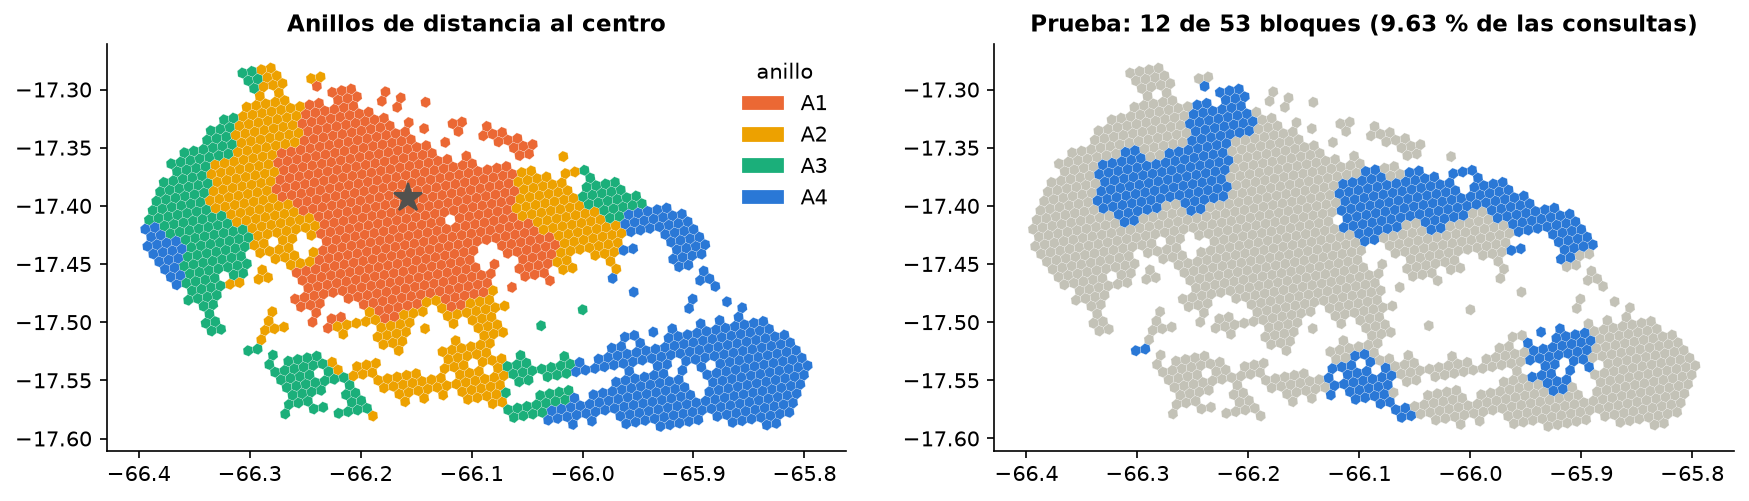
\includegraphics[width=\textwidth]{imagenes/07_desarrollo/7_3_preparacion/anillos_y_prueba.png}
  \fuente{Elaboración propia, a partir de \var{03_feature_engineering} (secciones 8 y 10).
  Izquierda: anillos A1 a A4 (la estrella marca la Plaza 14 de Septiembre); derecha: bloques
  de prueba en azul.}
\end{figure}

El desequilibrio entre zonas y consultas tiene una explicación, y debe tenerse en cuenta
al leer la evaluación. Los bloques del núcleo central, donde se concentra la mayor parte de
las consultas, quedaron del lado de entrenamiento. Por eso la tasa de la prueba (585
consultas por cada 1.000 habitantes) es un tercio de la de entrenamiento (1.913,6). La
prueba es, por tanto, más periférica y menos intensa que el conjunto con el que se
entrena. Es una condición exigente pero realista: la organización necesita estimaciones
confiables justamente en zonas alejadas del centro. Además, 125 de las 352 zonas de prueba
tocan zonas de entrenamiento en el borde de su bloque
(\var{zonas_prueba_borde} en \var{resultados/03_feature_engineering/metricas.json}). Es una
fuga mínima e inevitable en cualquier partición espacial, que se documenta y no se oculta.

El notebook termina con cuatro verificaciones automáticas:
\begin{itemize}
  \item la tabla conserva todas las consultas y no tiene nulos;
  \item los rangos de las variables son válidos;
  \item entrenamiento y prueba no comparten ningún bloque;
  \item ni el objetivo ni las variables GTFS figuran entre los predictores.
\end{itemize}
Los bloques reservados se guardan en \var{test_blocks.csv}. A partir de aquí, el notebook
de modelado solo los descarta y el de evaluación los usa una única vez.
